\documentclass[11pt]{article}
\usepackage[margin=1in]{geometry}
\usepackage[T1]{fontenc}
\usepackage{lmodern,microtype}
\usepackage{amsmath,amssymb,amsthm,mathtools}
\usepackage{booktabs,tabularx,longtable,array}
\usepackage{graphicx,xcolor,enumitem,fancyhdr}
\usepackage[hyphens]{url}
\usepackage{hyperref}
\definecolor{navy}{HTML}{17334B}
\definecolor{teal}{HTML}{087F8C}
\hypersetup{colorlinks=true,linkcolor=navy,citecolor=teal,urlcolor=teal,
 pdftitle={Finite spectral certificates and arithmetic determinant bounds},
 pdfauthor={Research note prepared for Vladimir Reshetnikov}}
\newcommand{\R}{\mathbb R}
\newcommand{\C}{\mathbb C}
\newcommand{\Z}{\mathbb Z}
\newcommand{\N}{\mathbb N}
\newcommand{\ind}{\mathbf 1}
\DeclareMathOperator{\tr}{tr}
\DeclareMathOperator{\ord}{ord}
\newtheorem{theorem}{Theorem}[section]
\newtheorem{lemma}[theorem]{Lemma}
\newtheorem{proposition}[theorem]{Proposition}
\newtheorem{corollary}[theorem]{Corollary}
\theoremstyle{definition}
\newtheorem{definition}[theorem]{Definition}
\theoremstyle{remark}
\newtheorem{remark}[theorem]{Remark}
\numberwithin{equation}{section}
\setlist{itemsep=3pt,topsep=5pt}
\setlength{\emergencystretch}{3em}
\setlength{\headheight}{14pt}
\pagestyle{fancy}
\fancyhf{}
\fancyhead[L]{\small Finite certificates and arithmetic determinants}
\fancyhead[R]{\small 26 November 2026}
\fancyfoot[C]{\thepage}
\title{\color{navy}\LARGE Finite spectral certificates and\par arithmetic determinant bounds\vspace{0.4em}\\
\large Results inspired by the \texttt{grh-lean} proof}
\author{Research note prepared for Vladimir Reshetnikov}
\date{26 November 2026}
\begin{document}
\maketitle
\begin{abstract}
We inspect the stated scope and two mechanisms of the current \texttt{grh-lean}
development: its smoothed prime-sum transform and its comparison of short
integral forms with determinant lower bounds. We derive and prove two
independent results inspired by these mechanisms.
First, a positive summable spectrum with integer multiplicities admits
finite certificates for complete cluster counts. A nonnegative polynomial
residual and weighted Hermite interpolation use only $2m+1$ consecutive
power moments for $m$ proposed clusters. We give explicit error constants,
rigorous propagation of approximate moment data, and eventual success of an
adaptive rational search at every threshold outside the spectrum. Under RH,
the spectrum $(\tfrac14+\gamma^2)^{-1}$ gives a zeta-zero application.
Second, for an integer $r\times n$ matrix, the Gram determinant divided by
the squared gcd of its maximal minors is at least
$\max\{N-z,\frac85N-4z,\frac{12}5N-12z\}$, where $N=\binom nr$ and $z$
counts vanishing maximal minors. The constants have exact equality examples.
An additional finite-factor surgery theorem explains why finite analytic
data cannot determine global simplicity in the larger class of real-zero
entire functions. Complete human-readable proofs and exact arithmetic
verification programs accompany this note. The formulations are derived
here; historical priority remains unestablished after a targeted literature
comparison. No full Lean formalization or independent rebuild of the RH
development is claimed.
\end{abstract}
\vspace{0.5em}
\noindent\textbf{Reading map.} Section~\ref{sec:spectral} contains the main
certificate theorem; Section~\ref{sec:zeta} explains its precise zeta
specialization. The determinant theorem is independent of RH.
The computational examples distinguish exact certificates from numerical
illustration.
\tableofcontents
\clearpage
\section{What the supplied sources establish}
\label{sec:sources}

The repository \texttt{lsernau/grh-lean} is pinned here to commit
\begin{center}
\small\texttt{72fead102f663d5c7a407964a13dc0cf9d977207}.
\end{center}
Its public interface proves Mathlib's \texttt{RiemannHypothesis} and four
explicit propositions about zeta and Dirichlet \(L\)-functions. The definitions
of those propositions import Mathlib alone; the auxiliary definitions used
inside the proof do not alter the exported statements~\cite{statements}.
The scope is as follows.

\begin{center}
\begin{tabularx}{\linewidth}{@{}lX@{}}
\toprule
Result & Mathematical content \\
\midrule
RH & Every nontrivial zero of \(\zeta\) has real part \(1/2\). \\
Dirichlet GRH & For every positive modulus and every Dirichlet character,
\(L(s,\chi)\ne0\) when \(\Re s>1/2\), with the principal-character pole excluded. \\
Critical-strip form & Every zero of any such \(L\)-function in
\(0<\Re s<1\) lies on \(\Re s=1/2\). \\
\bottomrule
\end{tabularx}
\end{center}

Primitive and imprimitive characters are included. This interface does not
assert GRH for arbitrary Artin or automorphic \(L\)-functions.
The repository pins Lean 4.35.0 and Mathlib commit
\nolinkurl{56a005855ea17e0b0958f73ec801ae140b0a1679}.
Its documentation reports compilation and independent checking, with only
\texttt{propext}, \texttt{Classical.choice}, and \texttt{Quot.sound} as axioms.
These are upstream verification reports; the present note does not provide a
fresh verification of the complete upstream development~\cite{repo}.
The supplied Wikipedia page describes the announced formal result and its
place among the classical formulations and consequences of RH~\cite{wiki}.

\subsection{A smoothing that exposes zero multiplicities}

One concrete mechanism is the conversion of a smoothed prime sum into a
meromorphic transform. For a suitable auxiliary prime \(d\), put
\(\chi_K(n)=(n/d)\) and
\[
 \lambda_{q,d}(n)=\Lambda(n)(1-\chi_K(n))\mathbf1_{n\equiv1\pmod q},
 \qquad
 R_{q,d}(x)=\sum_{n\le x}\lambda_{q,d}(n)
       \left(\frac1n-\frac1x\right)
       -\frac{\log x}{\varphi(q)}-c_{q,d}.
\]
The constant normalizes the remainder to tend to zero. Let \(E_\psi\) denote
\(L(s,\psi)\), with its principal pole removed when necessary. The transform
\[
 \int_0^\infty R_{q,d}(e^v)e^{(1-s)v}\,dv
\]
has, at \(\rho\ne0,1\), residue
\begin{equation}
 \frac{\displaystyle\sum_{\psi\bmod q}\operatorname{ord}_{\rho}E_\psi
       -\displaystyle\sum_{\psi\bmod q}\operatorname{ord}_{\rho}E_{\psi\chi_K}}
      {\varphi(q)\rho(1-\rho)}.
 \label{eq:source-residue}
\end{equation}
The source proves this by character orthogonality, partial summation, and
logarithmic derivatives~\cite{primeerror}.
For a critical-line zero \(\rho=1/2+i\gamma\), the denominator becomes
\(\rho(1-\rho)=1/4+\gamma^2\). Thus smoothing connects analytic data to
decaying positive weights on zero ordinates. The numerator in
\eqref{eq:source-residue} is a difference of multiplicities, so its positivity
requires additional information.

\subsection{The determinant comparison and the one-sided criterion}

The proof constructs integral forms with short theta-lift images, obtains
enough independent images through a second-moment argument, and compares
their Gram determinant with a lower bound from integrality. Auxiliary twists
may vary with the finite prime, while controlled determinant-ratio heights
link their valuations to the untwisted archimedean size~\cite{guide}.
Writing \(D\) for the target dimension and \(n\) for the selected independent
family size, the comparison has the schematic form
\[
 \text{main amount}
 \ \lesssim\ \frac{V+2\delta}{D}
 \ \lesssim\ \text{main amount}-\frac nD\,m\mathcal R,
\]
with explicitly controlled errors. Here \(V\) is a logarithmic squared
covolume and \(\delta\) is its index cost. Cancellation of the leading
quantity gives the exact bound
\begin{equation}
 m\mathcal R\le fa(\log b)^5.
 \label{eq:source-main}
\end{equation}
This is the theorem \texttt{star\_inequality}; its three principal inputs are
short forms, sufficiently many forms, and a lower bound for integral
forms~\cite{mainineq}.

The next reduction bounds
\[
 R_{q_0,d}(x)\le
 \frac{\varphi(q_0)(\log b)^6}{m}
 +|R_{q_0,d}(x_1)|+\log(b)|R_{1,d}(x_1)|.
\]
One chooses \(m\ge\sqrt{x}\), controls \(\log b\) by an arbitrarily small
power of \(x\), and uses the ordinary prime number theorem at the much larger
cutoff \(x_1\). This yields an eventual upper bound
\(R_{q_0,d}(x)\le x^{-1/2+\varepsilon}\) for every
\(\varepsilon>0\)~\cite{onesided}.
For any prospective zero with real part greater than \(1/2\), an appropriate
quadratic twist removes the unwanted twisted zeros in a finite-height
region. The remaining transform residues have the sign needed for a
Landau-type argument: the one-sided remainder bound forces them to vanish,
and their nonnegative multiplicities then vanish individually~\cite{criterion}.

The portable ideas used here are therefore precise: analytic smoothing
records zero multiplicities, and positivity converts moment or determinant
data into restrictions on zeros. The results below use the exported zero
location theorem and develop these ideas at the level of real-zero entire
functions. They do not extend the upstream automorphic construction to a
larger class of arithmetic \(L\)-functions.

\section{Complete cluster counts from a finite moment window}
\label{sec:spectral}

The first result isolates a useful form of discrete rigidity. A missed spectral
point contributes a definite positive amount to a carefully chosen residual.
Once the entire residual is smaller than that amount, the missed count must
be zero. A related interpolation construction recovers the integer count in
each proposed interval. The underlying spectrum may be infinite.

\subsection{Setup and the finite data}

Let $(x_n)$ be a finite or countably infinite multiset of positive real numbers,
with repeated values listed according to their positive integer multiplicities,
such that
\begin{equation}\label{eq:summability}
 p_1:=\sum_n x_n<\infty,
 \qquad p_j:=\sum_n x_n^j\quad(j\ge1).
\end{equation}
Every $x_n\le p_1$, so every $p_j$ is finite. There are only finitely many
occurrences above any positive threshold.

Choose $m\ge1$ distinct positive candidate centers $a_1,\ldots,a_m$, positive
radii $r_i<a_i$, and pairwise disjoint open intervals
\[
 I_i=(a_i-r_i,a_i+r_i).
\]
Fix an integer $K\ge1$. Define
\begin{align}
 P(x)&=\prod_{i=1}^m(x-a_i),
 &D_i&=\prod_{j\ne i}(a_i-a_j),\label{eq:P}\\
 L_i(x)&=\frac{\prod_{j\ne i}(x-a_j)}{D_i},
 &d_i&=\frac K{a_i}+2\sum_{j\ne i}\frac1{a_i-a_j},\label{eq:L}\\
 Q_i(x)&=\left(\frac x{a_i}\right)^K
       \bigl[1-d_i(x-a_i)\bigr]L_i(x)^2.\label{eq:Q}
\end{align}
Here and below empty products equal one and empty sums equal zero.
The residual and count estimates are
\begin{equation}\label{eq:RS}
 R_K=\sum_n x_n^K P(x_n)^2\ge0,
 \qquad S_i=\sum_n Q_i(x_n).
\end{equation}
They are absolutely convergent: each summand is a polynomial in $x_n$ with
no constant term, evaluated on a bounded summable spectrum.

The construction has three relevant properties:
\[
 Q_i(a_j)=\begin{cases}1,&j=i,\\0,&j\ne i,\end{cases}
 \qquad Q_i'(a_j)=0,
 \qquad x^K\mid Q_i(x).
\]
At $a_i$, the chosen linear factor cancels the logarithmic derivative
$K/a_i+2L_i'(a_i)$; at other centers, the squared factors give double zeros.
Moreover $\deg Q_i\le K+2m-1$ and $\deg(x^KP^2)=K+2m$. Thus all the
quantities in \eqref{eq:RS} use only the $2m+1$ moments
\begin{equation}\label{eq:window}
 p_K,p_{K+1},\ldots,p_{K+2m}.
\end{equation}
The number of entries in this window is fixed when $m$ is fixed. The starting
order $K$ and the required accuracy need not be small.

\subsection{Explicit count bounds}

For each $i$ set
\begin{align}
 b_i&=a_i-r_i,&g_{ij}&=|a_i-a_j|-r_i\quad(j\ne i),\\
 A_i&=\prod_{j\ne i}g_{ij}^{-2},
 &T_i&=\frac K{b_i}+2\sum_{j\ne i}g_{ij}^{-1},\\
 U_i&=\frac K{b_i^2}+2\sum_{j\ne i}g_{ij}^{-2}.&&
\end{align}
All $b_i,g_{ij}$ are positive by the interval assumptions. Put
\begin{equation}\label{eq:Ci}
 C_i=\max\left\{
 \frac{b_i^{-K}A_i}{2}(T_i^2+U_i),\quad
 \frac{a_i^{-K}}{D_i^2}\left(r_i^{-2}+|d_i|r_i^{-1}\right)
 \right\}.
\end{equation}

\begin{theorem}[Residual certificate]\label{thm:residual}
Under \eqref{eq:summability}, let $N_i$ count all occurrences in $I_i$,
with multiplicity. Then
\begin{equation}\label{eq:countbound}
 |N_i-S_i|\le C_iR_K.
\end{equation}
For any $\tau>0$, let $N_{\rm miss}$ count occurrences with $x_n\ge\tau$
outside $\bigcup_i I_i$. Then
\begin{equation}\label{eq:missing}
 N_{\rm miss}\le\frac{R_K}{\tau^K\prod_i r_i^2}.
\end{equation}
Consequently $R_K<\tau^K\prod_i r_i^2$ excludes every such missed point.
If, in addition to this strict no-missing inequality, the intervals lie
above $\tau$ and each interval
$[S_i-C_iR_K,S_i+C_iR_K]$ contains exactly one nonnegative integer $n_i$,
then the complete spectrum at or above $\tau$ is contained in these intervals
and has the exact cluster counts $(n_1,\ldots,n_m)$.
\end{theorem}

\begin{proof}
We first prove the pointwise estimate
\begin{equation}\label{eq:pointwise}
 |\ind_{I_i}(x)-Q_i(x)|\le C_i x^K P(x)^2\qquad(x>0).
\end{equation}
Outside $I_i$, write $u=x-a_i$, so $|u|\ge r_i$. Away from the other
candidate centers, cancellation gives
\[
 \frac{|Q_i(x)|}{x^KP(x)^2}
 =\frac{a_i^{-K}}{D_i^2}\frac{|1-d_iu|}{u^2}
 \le\frac{a_i^{-K}}{D_i^2}\left(r_i^{-2}+|d_i|r_i^{-1}\right).
\]
At another candidate center both sides of \eqref{eq:pointwise} are zero,
so the same inequality holds there by direct evaluation.

Inside $I_i$, there are no other candidate centers. Define the positive
smooth function $h_i(x)=x^{-K}L_i(x)^{-2}$. At the center,
\[
 h_i(a_i)=a_i^{-K},\qquad h_i'(a_i)=-d_i a_i^{-K}.
\]
Hence $Q_i(x)$ is $x^KL_i(x)^2$ times the first-degree Taylor polynomial
of $h_i$ at $a_i$, while $1=x^KL_i(x)^2h_i(x)$. Since
$P(x)=(x-a_i)D_iL_i(x)$, Taylor's theorem with integral remainder gives
\[
 \frac{|1-Q_i(x)|}{x^KP(x)^2}
 \le\frac1{2D_i^2}\sup_{t\in I_i}|h_i''(t)|
 \quad(x\ne a_i).
\]
Logarithmic differentiation yields the exact expression
\begin{align*}
 \frac{h_i''(t)}{D_i^2}
 &=t^{-K}\prod_{j\ne i}(t-a_j)^{-2}\times{}\\[-2pt]
 &\quad\left\{
 \left(\frac Kt+2\sum_{j\ne i}\frac1{t-a_j}\right)^2
 +\frac K{t^2}+2\sum_{j\ne i}\frac1{(t-a_j)^2}\right\}.
\end{align*}
It is nonnegative and at most $b_i^{-K}A_i(T_i^2+U_i)$, using
$t\ge b_i$ and $|t-a_j|\ge g_{ij}$. At $x=a_i$, both sides of
\eqref{eq:pointwise} vanish. This proves the pointwise bound everywhere.

Absolute convergence permits summation of \eqref{eq:pointwise}, proving
\eqref{eq:countbound}. Every missed occurrence has $x_n\ge\tau$ and
$|x_n-a_i|\ge r_i$ for all $i$, and therefore contributes at least
$\tau^K\prod_i r_i^2$ to $R_K$. Summing gives \eqref{eq:missing}.
A nonnegative integer smaller than one is zero. Finally the true integer
$N_i$ must lie in its certified interval, giving the exact counts.
\end{proof}

\begin{remark}[What a cluster count means]
A count of one proves that the interval contains one simple spectral
occurrence. A count greater than one may represent a repeated value or
several distinct nearby values. No assumption of simple zeros is used.
The no-missing conclusion also excludes spectral points at the interval
endpoints, because the intervals are open.
\end{remark}

\subsection{Certified errors in the input moments}

Write
\[
 x^KP(x)^2=\sum_{j=K}^{K+2m}u_jx^j,
 \qquad Q_i(x)=\sum_{j=K}^{K+2m}v_{ij}x^j,
\]
where the final coefficient of $Q_i$ is zero. Suppose the input satisfies
$|p_j-\widehat p_j|\le\epsilon_j$. Compute
\begin{align}
 \widehat R&=\sum_j u_j\widehat p_j,
 &R^+&=\widehat R+\sum_j|u_j|\epsilon_j,\\
 \widehat S_i&=\sum_jv_{ij}\widehat p_j,
 &E_i&=\sum_j|v_{ij}|\epsilon_j.
\end{align}

\begin{corollary}[Robust finite verification]\label{cor:noise}
Valid input enclosures imply $0\le R_K\le R^+$ and
\[
 |N_i-\widehat S_i|\le E_i+C_iR^+,
 \qquad N_{\rm miss}\le\frac{R^+}{\tau^K\prod_i r_i^2}.
\]
Thus the no-missing test with $R^+$ and a unique integer in each enlarged
count interval constitute a rigorous certificate. One sufficient rounding
test, for a proposed integer $n_i\ge0$, is
\[
 |\widehat S_i-n_i|+E_i+C_iR^+<\frac12.
\]
All verification operations are rational when the centers, radii, threshold,
moment midpoints and error bounds are rational.
\end{corollary}
\begin{proof}
The triangle inequality bounds the errors in both linear moment functionals.
Substitute these bounds into Theorem~\ref{thm:residual}.
\end{proof}

If $R^+<0$, the supplied enclosures contradict the nonnegative residual and
must be rejected. A verifier must not silently replace a negative upper
bound by zero. The input enclosures themselves remain a mathematical
premise: passing this verifier cannot validate arbitrary untrusted moment
data.

\subsection{Why a fixed-width certificate eventually exists}

\begin{theorem}[Eventual certificates]\label{thm:eventual}
Let $\tau>0$ be outside the spectrum. Let $m$ be the number of distinct
spectral values above $\tau$. There is a certificate of the preceding form
using $2m+1$ consecutive moments, with rational candidate centers and radii
in arbitrarily narrow disjoint intervals about those values. If $\tau$ is
rational and the moments can be approximated with certified errors to any
requested precision, an exhaustive rational search eventually finds a
complete correct certificate above $\tau$.
\end{theorem}

\begin{proof}
First let $m\ge1$ and take the candidate centers to be the actual distinct
spectral values above $\tau$. Choose narrow disjoint intervals with
$b_i=a_i-r_i>\tau$. Summability implies that every compact subinterval of
$(0,\infty)$ contains only finitely many spectral occurrences. Since $\tau$
is not a spectral value, all remaining occurrences lie in $(0,\sigma]$ for
some $0<\sigma<\tau$. Write $S_{\rm tail}$ for their first moment.

At the leading spectral values $P$ vanishes exactly. For $0\le x\le\sigma$,
each $a_i>\sigma$, so $P(x)^2\le\prod_i a_i^2$. Therefore
\begin{equation}\label{eq:taildecay}
 R_K\le S_{\rm tail}\,\sigma^{K-1}\prod_i a_i^2.
\end{equation}
For fixed centers and radii, \eqref{eq:Ci} gives
$C_i=O((K+1)^2b_i^{-K})$. Because $\sigma<\tau<b_i$,
\[
 \frac{R_K}{\tau^K\prod_i r_i^2}\longrightarrow0,
 \qquad C_iR_K\longrightarrow0.
\]
The exact integer counts then satisfy the sufficient rounding inequality for
all sufficiently large $K$: indeed
$|S_i-N_i|+C_iR_K\le2C_iR_K\to0$.

Fix one such $K$ with strict slack. The finite formulas are continuous in
the distinct centers, positive admissible radii, and moments. Choose
rational centers and radii sufficiently close to the original ones; their
intervals still enclose the same spectral values. Then choose sufficiently
accurate rational moment enclosures. All strict certificate inequalities
persist. The interval widths may have been arbitrarily small from the start.

When $m=0$, choose $\sigma<\tau$ bounding the entire spectrum. The simple
test $p_K<\tau^K$ eventually holds, since
$p_K\le p_1\sigma^{K-1}$. It certifies that the count above $\tau$ is zero.

Finally enumerate finite rational configurations, positive integers $K$,
and requested moment precisions. For each configuration, the tests of
Corollary~\ref{cor:noise} terminate using rational arithmetic. Dovetailing
this enumeration eventually reaches one of the certificates just proved
to exist. This is an existence and termination argument, not an efficiency
bound.
\end{proof}

\begin{remark}[Conditioning is visible in the theorem]
The proof does not say that fixed approximate centers improve indefinitely
as $K$ grows. Suppose actual leading values $\lambda_i\le B$ have total
multiplicity $M$, $|a_i-\lambda_i|\le\eta$, and the tail is bounded by
$\sigma<\min_i a_i$. A direct product estimate gives
\[
 R_K\le MB^K\eta^2(2B+\eta)^{2m-2}
       +S_{\rm tail}\sigma^{K-1}\prod_i a_i^2.
\]
The first term can require increasingly accurate centers at larger $K$.
Small separation between different centers also enlarges $D_i^{-2}$ and
the $g_{ij}^{-1}$ factors. The explicit constants record this cost.
\end{remark}

\section{The zeta and Dirichlet applications}\label{sec:zeta}

Define
\[
 \xi(s)=\tfrac12s(s-1)\pi^{-s/2}\Gamma(s/2)\zeta(s),
 \qquad \Xi(t)=\xi(\tfrac12+it).
\]
The standard completion satisfies $\xi(s)=\xi(1-s)$ and is entire
\cite{dlmf,cardon}. Use RH, as provided by the inspected development, and list
positive zero ordinates $\gamma_n$ with multiplicity. Set
\begin{equation}\label{eq:zetanodes}
 x_n=\frac1{\tfrac14+\gamma_n^2}.
\end{equation}
This is precisely the positive denominator arising from
$\rho(1-\rho)$ in the repository's transform reduction.

\begin{proposition}[Moment coordinate]\label{prop:xi}
The symmetry quotient
\begin{equation}\label{eq:H}
 H(z)=2\xi\!\left(\frac{1+\sqrt{1+4z}}2\right)
\end{equation}
is a single-valued entire function, despite the square-root notation. It has
the locally uniformly convergent product
\begin{equation}\label{eq:Hproduct}
 H(z)=\prod_n(1+x_nz),\qquad H(0)=1.
\end{equation}
Consequently, for the analytic logarithm at zero,
\begin{equation}\label{eq:logmoments}
 p_j=(-1)^{j-1}j[z^j]\log H(z)
     =\frac{(-1)^{j-1}}{(j-1)!}(\log H)^{(j)}(0),
\end{equation}
and
\begin{equation}\label{eq:p1}
 p_1=1+\frac{\gamma_{\!E}}2-\frac12\log(4\pi).
\end{equation}
\end{proposition}

\begin{proof}
The entire function $w\mapsto\xi(\tfrac12+w)$ is even. Its power series
is therefore an entire power series in $w^2$. Substituting $w^2=z+\tfrac14$
proves that \eqref{eq:H} is entire and independent of the square-root choice.
The paired Hadamard product under RH is
\[
 \xi(\tfrac12+w)=\xi(\tfrac12)
       \prod_{\gamma_n>0}\left(1+\frac{w^2}{\gamma_n^2}\right).
\]
Pairing the genus-one factors removes their exponential factors, while
evenness removes the possible linear exponential prefactor. The usual
order-one factorization gives $\sum_n\gamma_n^{-2}<\infty$. There is no
central zeta zero; for example the alternating eta series at $1/2$ is
positive while $1-\sqrt2<0$, so $\zeta(1/2)\ne0$.

Divide the paired product at $w^2=z+\tfrac14$ by its value at
$w^2=\tfrac14$. Since $\xi(1)=\tfrac12$, this gives
\[
 2\xi(\tfrac12+w)
 =\prod_n\frac{\gamma_n^2+w^2}{\gamma_n^2+\tfrac14},
\]
which is \eqref{eq:Hproduct}. Summability justifies taking the logarithmic
power series near zero, proving \eqref{eq:logmoments}. Finally
$H'(0)/H(0)=\xi'(1)/\xi(1)$. Substitute the Laurent expansion
$\zeta(1+u)=u^{-1}+\gamma_E+O(u)$ into the defining completion, together
with $\Gamma'(1/2)/\Gamma(1/2)=-\gamma_E-2\log2$, to obtain
\eqref{eq:p1}.
\end{proof}

\begin{corollary}[Complete zeta-zero cluster certificates]\label{cor:zeta}
Use certified moment enclosures from \eqref{eq:logmoments}. Suppose
$0<\tau<a_i-r_i<a_i+r_i<4$, and the tests of
Corollary~\ref{cor:noise} succeed. Then every positive-ordinate nontrivial
zeta zero with
\[
 \gamma\le T:=\sqrt{\tau^{-1}-\tfrac14}
\]
lies in one of the disjoint intervals
\begin{equation}\label{eq:gammawindows}
 J_i=\left(
 \sqrt{(a_i+r_i)^{-1}-\tfrac14},\quad
 \sqrt{(a_i-r_i)^{-1}-\tfrac14}\right).
\end{equation}
The certified integer $n_i$ is the number of zeros in $J_i$, counting
multiplicity, and the total count is $\sum_i n_i$. If the threshold is not
a spectral value, arbitrarily narrow such certificates exist.
\end{corollary}
\begin{proof}
The map $x\mapsto\sqrt{x^{-1}-1/4}$ is decreasing on $(0,4)$ and carries
\eqref{eq:zetanodes} back to the positive ordinates. Apply the preceding
theorems. The threshold and boundary exclusions are supplied by the
no-missing certificate.
\end{proof}

For numerical conditioning it is convenient to use $y_n=cx_n$ for a
positive scale $c$. Replace $H(z)$ by $H(cz)$ and replace $x^{-1}$ in
\eqref{eq:gammawindows} by $c/y$. All abstract formulas are unchanged.

\subsection{Scope of the Dirichlet extension}

The abstract theorem applies to any positive trace-class spectrum with
integer multiplicities, using $p_j=\tr(T^j)$. Its Dirichlet application is
also straightforward once the spectral count convention is fixed.
For a primitive nonprincipal character $\chi$, form the product of the
completed $L$-functions for $\chi$ and $\overline\chi$. Their functional
equations make the product even about $s=1/2$. Under Dirichlet GRH its
noncentral zeros lie on that line. Remove its central factor first, and
apply the even paired canonical product as above. The resulting positive
moments certify combined noncentral zero counts for the pair.

For a real character, using the character twice doubles those counts; one
can instead use the appropriately normalized single completion after
removing its central zero. The zeta completion handles the primitive
principal character. Imprimitive characters should be reduced to their
primitive inducing characters, treating their additional Euler factors
separately. Central vanishing is not excluded by Dirichlet GRH and must
not be silently discarded. We do not claim that the inspected repository
proves GRH for all automorphic or Artin $L$-functions.

\subsection{Relation to earlier reconstruction results}

Finite moment reconstruction and polynomial dual certificates are
established methods. De Castro and Gamboa prove recovery of a nonnegative
measure on $s$ points from $2s+1$ generalized moments \cite{decg}.
Batenkov and Yomdin quantify the conditioning of finite Prony systems
\cite{prony}; Cand\`es and Fernandez-Granda give stable recovery results
from noisy bandlimited data under separation hypotheses \cite{superres}.
Cardon and de Gaston connect orthogonal polynomials to RH with simple
zeros \cite{cardon}.

A particularly close recent comparison is \emph{A finite arithmetic test
for simplicity of the Riemann zeros, after Suzuki} \cite{ald}. It compares
multiplicity-weighted Taylor moments with finite operator-compression
traces to detect excess multiplicity. The present certificate uses direct
positive moments, a candidate polynomial, and scalar Hermite bounds to
certify complete cluster counts. It makes no distinction between a repeated
root and multiple roots within a cluster of count greater than one.

The specific contribution proposed here is the combination of an infinite
summable integer spectrum, an explicit residual and count constant, a
fixed-width shifted moment window, rigorous input-error propagation, and
eventual rational certificates. None of the cited classical ingredients is
claimed as new, and the literature search does not establish priority for
the combined formulation.

\section{Arithmetic determinant bounds with vanishing minors}
\label{sec:determinants}

The repository organizes its central comparison around short integral
forms, enough forms to span, and a lower bound saying that integral forms
are long; determinants combine these inputs
\cite{guide,mainineq}. This suggests an independent finite-dimensional
question. How small can an integer matrix's Gram determinant be when
many of its maximal minors are nonzero? Integrality gives one lower
bound, but the algebraic relations between minors force a stronger one.
The result below also quantifies what remains when some minors vanish.
It is unconditional and does not use RH.

\begin{theorem}[Arithmetic determinant amplification]
\label{thm:determinant}
Let $A\in\Z^{r\times n}$ have row rank $r$, where $n\ge5$ and
$2\le r\le n-2$. For an $r$-element subset $B\subseteq\{1,\ldots,n\}$,
write $A_B$ for the square matrix formed by its columns in increasing
order. Define
\[
 N=\binom nr,\qquad
 z=\#\{B:\det A_B=0\},\qquad
 D=\gcd\{\lvert\det A_B\rvert:\det A_B\ne0\}.
\]
Then $D>0$ and
\begin{equation}
\boxed{\quad
 \frac{\det(AA^{\mathsf T})}{D^2}
 \ge
 \max\left\{N-z,\ \frac85N-4z,\ \frac{12}5N-12z\right\}.
 \quad}
\label{eq:det-main}
\end{equation}
In particular, if every $r$ columns are linearly independent, then
\begin{equation}
 \det(AA^{\mathsf T})\ge\frac{12}{5}\binom nr D^2.
 \label{eq:det-generic}
\end{equation}
The coefficient $12/5$ in \eqref{eq:det-generic} cannot be increased
uniformly over this class. Each of the three affine inequalities in
\eqref{eq:det-main} has equality examples.
\end{theorem}

The statement does not assert that the maximum in
\eqref{eq:det-main} is optimal for every fixed triple $(r,n,z)$.
For comparison, Cauchy--Binet and integrality alone give only $N-z$.
The stronger terms come from the Pl\"ucker relations, which prohibit
an integral system of minors from having too many small absolute values.

\subsection{Two local obstructions}

For four labels, the relevant relation is
\begin{equation}
 p_{12}p_{34}-p_{13}p_{24}+p_{14}p_{23}=0.
 \label{eq:det-plucker}
\end{equation}
It holds for the two-row minors of any matrix, by direct expansion.
We shall use integer coordinate systems satisfying this relation on
each four-element set of labels.

\begin{lemma}[Four nonvanishing labels]
\label{lem:det-four}
If the six integers in \eqref{eq:det-plucker} are all nonzero, then
\[
 \sum_{1\le i<j\le4}p_{ij}^{,2}\ge9.
\]
\end{lemma}
\begin{proof}
If all six absolute values were one, the left side of
\eqref{eq:det-plucker} would be a sum of three signed ones and could
not vanish. One squared coordinate is therefore at least four; the
other five are at least one.
\end{proof}

\begin{lemma}[Five nonvanishing labels]
\label{lem:det-five}
Suppose the ten integers $p_{ij}$, $1\le i<j\le5$, are nonzero and
satisfy the Pl\"ucker relation on every four-element set. Then
\begin{equation}
 \sum_{1\le i<j\le5}p_{ij}^{,2}\ge24.
 \label{eq:det-local24}
\end{equation}
\end{lemma}
\begin{proof}
Suppose the sum is at most $23$. No coordinate has absolute value at
least four, since that would contribute at least $16+9=25$ in total.
There is at most one coordinate of absolute value three, since two
would contribute at least $18+8=26$.

If the edge $\{a,b\}$ has absolute value three, there is at most one
edge of absolute value two: relative to the baseline sum $10$, the
three contributes an excess of $8$ and two twos would contribute
another $6$. Choose four labels containing $\{a,b\}$ but excluding
the possible edge of absolute value two. To do this, omit an endpoint
of the latter edge outside $\{a,b\}$. The three absolute products in
the resulting relation are $3,1,1$, which cannot have a signed sum
equal to zero. Hence no coordinate has absolute value three.

All absolute values are consequently one or two. Call an edge
\emph{heavy} when its absolute value is two. On any four labels,
the three absolute products belong to $\{1,2,4\}$. A signed sum of
three nonzero real numbers can vanish only when one absolute value
equals the sum of the other two. The only possible product multisets
are therefore
\[
 \{2,1,1\}\qquad\text{or}\qquad\{4,2,2\}.
\]
Their products show that the six edges contain, respectively, one or
four heavy edges. There are five four-label subsets, and every edge
belongs to three of them. If $h$ is the number of heavy edges and $k$
the number of four-label subsets with four heavy edges, double counting
gives
\[
 3h=(5-k)+4k=5+3k,
\]
a contradiction modulo three.
\end{proof}

\begin{lemma}[Five labels with zeros]
\label{lem:det-five-defect}
For ten integer Pl\"ucker coordinates on five labels, let $w$ count
the zero coordinates and let $V$ be their sum of squares. Then
\begin{equation}
 V\ge\max\{10-w,\ 16-4w,\ 24-12w\}.
 \label{eq:det-local-defect}
\end{equation}
\end{lemma}
\begin{proof}
Integrality gives $V\ge10-w$. If $w=0$,
Lemma~\ref{lem:det-five} gives $V\ge24$. If $w=1$, delete an endpoint
of the unique zero edge. The six coordinates on the remaining four
labels are nonzero and contribute at least nine by
Lemma~\ref{lem:det-four}. The three other nonzero coordinates contribute
at least three more, giving $V\ge12$.

These two cases prove $V\ge24-12w$, since its right side is
nonpositive for $w\ge2$. They also prove $V\ge16-4w$ for $w=0,1$.
For $w\ge2$, the baseline bound suffices because
$10-w\ge16-4w$.
\end{proof}

\subsection{From local relations to all maximal minors}

\begin{proof}[Proof of Theorem~\ref{thm:determinant}]
Put $p_B=\det(A_B)/D\in\Z$. Cauchy--Binet gives
\begin{equation}
 S:=\frac{\det(AA^{\mathsf T})}{D^2}
   =\sum_{|B|=r}p_B^2.
 \label{eq:det-cb}
\end{equation}

First suppose $r\le n-3$. Choose disjoint index sets $I,J$ with
$|I|=r-2$ and $|J|=5$. For distinct $a,b\in J$, define
\[
 q_{ab}=D^{-1}\det(A_{I,a,b}),
\]
where the columns in $I$ are listed increasingly and followed by
$a,b$ in that order. These are signed versions of the coordinates
$p_{I\cup\{a,b\}}$. They satisfy the four-label Pl\"ucker relations.
Indeed, if the columns indexed by $I$ are dependent, all $q_{ab}$
vanish. Otherwise an invertible real row change sends these columns
to the first $r-2$ standard basis vectors. Expansion in those columns
expresses the $q_{ab}$ as a common real multiple of two-row minors;
the relation follows from \eqref{eq:det-plucker} and its homogeneity.

Let $V_{I,J}$ and $w_{I,J}$ be the local sum of squares and number of
zeros. The number of local systems is
\[
 L=\binom n{r-2}\binom{n-r+2}{5}.
\]
Each global coordinate $p_B$ occurs in exactly
\[
 t=\binom r2\binom{n-r}{3}>0
\]
local systems: choose the two elements of $B$ outside $I$, then the
three elements of $J$ outside $B$. Counting all occurrences gives
\[
 10L=Nt,\qquad
 \sum_{I,J}V_{I,J}=tS,\qquad
 \sum_{I,J}w_{I,J}=tz.
\]
Sum each of the three separate affine inequalities in
\eqref{eq:det-local-defect}, then divide by $t$. Substituting
$10L=Nt$ yields
\[
 S\ge N-z,\qquad
 S\ge\frac85N-4z,\qquad
 S\ge\frac{12}5N-12z.
\]

Finally, suppose $r=n-2$. The complementary coordinates
\[
 p^*_{ij}=\pm p_{\{1,\ldots,n\}\setminus\{i,j\}}
 \qquad(i<j),
\]
with signs given by the complement permutation, form a decomposable
rank-two Pl\"ucker system. To see this directly, take a basis of the
two-dimensional orthogonal complement of the row space of $A$.
Laplace expansion identifies its two-row minors, up to one common
nonzero real factor, with the signed complementary maximal minors
of $A$. Hence the $p^*_{ij}$ satisfy the rank-two relations. They
are integers and preserve both the sum of squares and the number
of zeros, while $\binom n2=\binom nr=N$. Apply the rank-two argument
just proved. This establishes \eqref{eq:det-main} in all cases.
The equality examples below prove the sharpness assertions.
\end{proof}

\subsection{Equality, an energy obstruction, and scope}

Write
\[
 e_1=(1,0)^{\mathsf T},\quad e_2=(0,1)^{\mathsf T},\quad
 u=(1,1)^{\mathsf T},\quad v=(1,-1)^{\mathsf T},\quad
 w=(1,2)^{\mathsf T}.
\]
The following matrices all have $r=2$, $n=5$, $N=10$, and $D=1$:
\begin{center}
\renewcommand{\arraystretch}{1.3}
\begin{tabular}{c l c c}
\hline
$z$ & Columns of $A$ & $AA^{\mathsf T}$ & $S$\\
\hline
$0$ & $e_1,e_2,u,v,w$ & $\left(\begin{smallmatrix}4&2\\2&7\end{smallmatrix}\right)$ & $24$\\
$1$ & $e_1,e_1,e_2,u,v$ & $\left(\begin{smallmatrix}4&0\\0&3\end{smallmatrix}\right)$ & $12$\\
$2$ & $e_1,e_1,e_2,e_2,u$ & $\left(\begin{smallmatrix}3&1\\1&3\end{smallmatrix}\right)$ & $8$\\
$3$ & $e_1,e_1,e_1,e_2,u$ & $\left(\begin{smallmatrix}4&1\\1&2\end{smallmatrix}\right)$ & $7$\\
\hline
\end{tabular}
\end{center}
The first example attains $12N/5-12z$; the second attains both
nontrivial affine bounds; the third attains $8N/5-4z$ and the baseline;
the fourth attains the baseline alone. Complementary minors give the
rank-three equality example
\[
 B=\begin{pmatrix}
 -1&-1&1&0&0\\
 -1& 1&0&1&0\\
 -1&-2&0&0&1
 \end{pmatrix},
 \qquad \det(BB^{\mathsf T})=24.
\]
Its rows form an integer basis of the kernel of the first two-row
example, and its ten maximal minors are all nonzero with gcd one.

If $\delta=z/N$, the normalized lower bound is
\begin{equation}
 \frac{S}{N}\ge
 \begin{cases}
 12/5-12\delta,&0\le\delta\le1/10,\\
 8/5-4\delta,&1/10\le\delta\le1/5,\\
 1-\delta,&1/5\le\delta\le1.
 \end{cases}
 \label{eq:det-density}
\end{equation}
\begin{figure}[htbp]
\centering
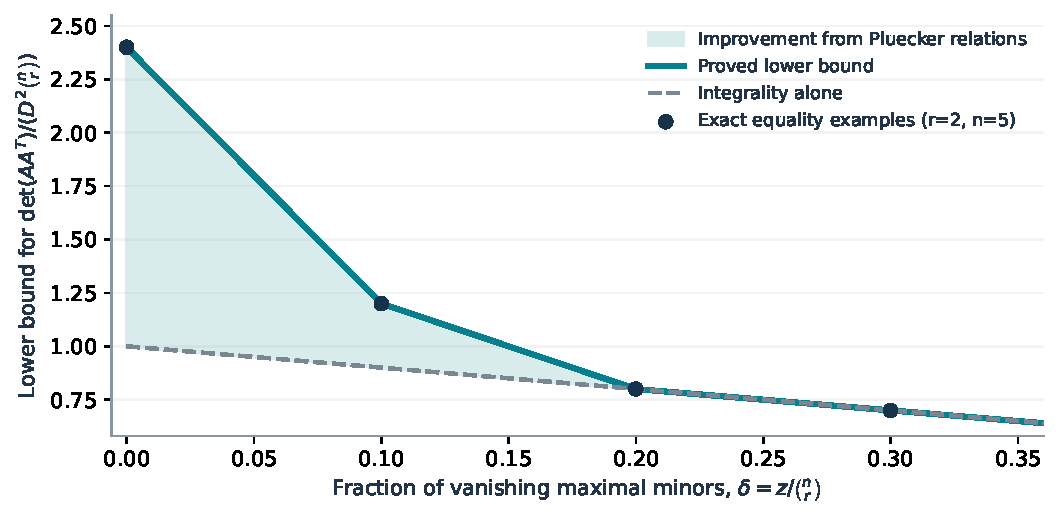
\includegraphics[width=.85\linewidth]{figures/determinant_bound.pdf}
\caption{The proven determinant lower bound as a function of the
fraction of vanishing maximal minors. The marked equality examples
have $n=5$ and $r=2$; the curve is a universal lower bound, not a
claim of optimality for every fixed dimension and zero count.}
\label{fig:det-bound}
\end{figure}

\begin{corollary}[A quantitative obstruction to short integral columns]
\label{cor:det-energy}
Under the hypotheses of Theorem~\ref{thm:determinant}, put
$E=\sum_{j=1}^n\|A_j\|^2$ and
$F=\max\{N-z,8N/5-4z,12N/5-12z\}$. Then
\[
 E\ge rD^{2/r}F^{1/r}.
\]
If every maximal minor is nonzero and every column has length at
most $H$, necessarily
\[
 \left(\frac{nH^2}{r}\right)^r\ge\frac{12}5\binom nr D^2.
\]
\end{corollary}
\begin{proof}
The positive eigenvalues of $AA^{\mathsf T}$ have sum $E$.
The arithmetic--geometric mean inequality gives
$(E/r)^r\ge\det(AA^{\mathsf T})$. Apply
Theorem~\ref{thm:determinant}, and use $E\le nH^2$ in the last case.
\end{proof}

This corollary makes the methodological connection precise: common
determinantal divisibility, many independent column subsets, and small
total squared length impose competing requirements. It does not by
itself improve the repository's RH proof. Such an application would
require matching its forms and lattices to the matrix hypotheses and
normalization used here.

The closest literature located concerns generic integer matrices with
bounded largest maximal minor and their maximal number of columns
\cite{generic2023,generic2025}. In particular, the weaker fact that a
generic two-row five-column integer matrix must have a minor of absolute
value at least three is already known. The proposed contribution here
is the aggregate sum-of-squares inequality, its explicit dependence on
vanishing minors, and the local proof with equality examples. A targeted
literature search did not locate this formulation; it does not establish
priority. The supplied exact-arithmetic script verifies all five
displayed examples, independently of the human proof above.

\section{Exact finite-jet surgery with a prescribed multiple zero}
\label{sec:surgery}

Finite moment information can certify useful local statements, but it cannot
by itself force global simplicity. The following theorem gives a precise
obstruction while preserving reality of all zeros and even the eventual
zero-counting function. Its algebraic ingredient is the classical inversion
of consecutive power sums~\cite{powersums}.

\begin{theorem}[Finite-jet surgery]
\label{thm:surgery}
Let
\[
 F(z)=F(0)\prod_{n\ge1}(1-a_nz^2),\qquad
 F(0)\in\mathbb R\setminus\{0\},\quad a_n>0,\quad\sum_n a_n<\infty,
\]
with infinitely many distinct nodes \(a_n\); factors are listed with
multiplicity. Fix integers \(d,r\ge1\), choose \(d\) distinct anchor nodes
\(a_1,\ldots,a_d\), and let \(\epsilon>0\).
There exists \(L>0\) such that, for any \(r\) other factor occurrences with
positive zero ordinates \(\beta_1,\ldots,\beta_r\ge L\), and any
\(T\ge L\) with \(F(T)\ne0\), there are positive distinct nodes \(u_i\)
satisfying \(|u_i-a_i|<\epsilon\) for which
\begin{equation}
 G(z)=F(z)
 \frac{\prod_{i=1}^d(1-u_i z^2)(1-z^2/T^2)^r}
 {\prod_{i=1}^d(1-a_i z^2)\prod_{j=1}^r(1-z^2/\beta_j^2)}
 \label{eq:surgery-function}
\end{equation}
has the following properties:
\begin{enumerate}[label=\textup{(\roman*)},nosep]
\item \(G\) is even and entire, is real on the real axis, and has only real
zeros. Its zeros at \(T\) and \(-T\) have multiplicity exactly \(r\).
\item \(G(0)=F(0)\) and \(G-F=O(z^{2d+2})\). The first \(d\)
nonconstant logarithmic Taylor coefficients agree exactly.
\item If \(N_H(Y)\) counts positive zeros of \(H\) up to \(Y\), with
multiplicity, then \(|N_G(Y)-N_F(Y)|\le d+r\) for every \(Y\ge0\), and
\(N_G(Y)=N_F(Y)\) for all sufficiently large \(Y\).
\item With \(M_H(R)=\max_{|z|=R}|H(z)|\), one has
\(\log M_G(R)-\log M_F(R)=O(1)\). In particular order and growth type
are preserved.
\end{enumerate}
\end{theorem}

\begin{proof}
Write \(b_j=\beta_j^{-2}\), \(c=T^{-2}\), and consider the power-sum map
\[
 \Phi(u)=\left(\sum_{i=1}^d u_i^k\right)_{k=1}^d.
 \qquad
 \det D\Phi(a)=d!\prod_{i<j}(a_j-a_i)\ne0.
\]
The real inverse function theorem gives a neighborhood of \(\Phi(a)\)
whose points have preimages in arbitrarily small disjoint positive intervals
about the anchors. We seek
\begin{equation}
 \sum_i u_i^k=\sum_i a_i^k+\sum_j b_j^k-r c^k,
 \qquad 1\le k\le d.
 \label{eq:surgery-moments}
\end{equation}
If \(b_j,c\le\eta\le1\), each perturbation on the right has absolute
value at most \(r\eta^k\le r\eta\). Choosing \(\eta\) small enough and
\(L\ge\eta^{-1/2}\) therefore solves every such system. Increase \(L\)
to exceed the anchor ordinates and all their permitted perturbations.

The denominator factors in \eqref{eq:surgery-function} are factors of
\(F\), so the quotient is entire. The new positive node sequence still
has finite sum; its product converges locally uniformly and has precisely
the stated real zeros. Since \(F(T)\ne0\), the new multiplicity is exactly
\(r\). Near zero, absolute convergence gives
\[
 \log\frac{F(z)}{F(0)}
   =-\sum_{k\ge1}\frac{z^{2k}}k\sum_n a_n^k.
\]
Equation \eqref{eq:surgery-moments} cancels the first \(d\) terms of
\(\log(G/F)\). Exponentiating proves \(G-F=O(z^{2d+2})\), hence equality
of derivatives through order \(2d+1\).

Exactly \(d+r\) positive zero occurrences were deleted and the same number
inserted. Their finite cumulative counts differ by at most \(d+r\), and
agree beyond the largest changed ordinate. Finally,
\[
 \frac{G(z)}{F(z)}\longrightarrow
 \frac{c^r\prod_i u_i}{\prod_i a_i\prod_j b_j}>0
 \qquad(|z|\to\infty).
\]
Outside a sufficiently large disk this rational quotient is bounded above
and below in modulus by positive constants. The same bounds hold for the
ratio of maximum moduli, proving \textup{(iv)}.
\end{proof}

\paragraph{A finite constructive certificate.}
The inverse function theorem can be replaced by Newton's identities and
endpoint signs. Set
\[
 q_k=\sum_i a_i^k+\sum_jb_j^k-r c^k,\qquad
 e_0=1,\qquad e_k=\frac1k\sum_{j=1}^k(-1)^{j-1}e_{k-j}q_j,
\]
and form
\[
 P_q(X)=X^d-e_1X^{d-1}+\cdots+(-1)^d e_d.
\]
At \(b_j=c=0\), this is \(P_0(X)=\prod_i(X-a_i)\). Choose disjoint
positive intervals \([\ell_i,h_i]\) around the anchors. Their endpoint
signs are opposite. For small enough \(b_j,c\), coefficient continuity
preserves every endpoint sign. The intermediate value theorem gives a root
in each interval; degree \(d\) forces all these roots to be simple and to
exhaust the roots of \(P_q\). Newton's identities then give
\eqref{eq:surgery-moments} exactly. In particular, the sufficient check
\[
 \sum_{j=1}^d|e_j(q)-e_j(\Phi(a))|B^{d-j}<m,
 \quad
 B=\max_i(1,|\ell_i|,|h_i|),\quad
 m=\min_i\bigl(|P_0(\ell_i)|,|P_0(h_i)|\bigr)
\]
certifies the construction by finite arithmetic. Rational input and rational
endpoints give an exact rational certificate.

\paragraph{Protected zeros and compact approximation.}
The anchors can be chosen above any fixed height \(H\), with perturbation
intervals staying above \(H\); the zero multiset in \([-H,H]\) is then
unchanged. One can also require \(\sup_{|z|\le R}|G(z)-F(z)|<\delta\) for
any fixed \(R,\delta>0\). Indeed, write
\(F=H_a\prod_i(1-a_i z^2)\) with \(H_a\) entire. As the high nodes
\(b_j,c\) tend to zero, \(u_i\to a_i\) and
\((1-cz^2)^r/\prod_j(1-b_jz^2)\to1\) uniformly on the disk. This
factorization also handles disks containing the moved anchor zeros.
The same argument plants any fixed finite multiplicity pattern at
sufficiently high targets.

\paragraph{An explicit example.}
Let \(F(t)=\sin(\pi t)/(\pi t)\). Use the zeros \(1,2\) as anchors,
delete \(10,11\), and plant a double zero at \(T=25/2\). Put
\[
 q_1=\frac{189889}{151250},\qquad
 e_2=\frac{194206753}{756250000},\qquad
 P(X)=X^2-q_1X+e_2.
\]
Its discriminant is \(3139703802/5719140625>0\). Opposite endpoint signs
locate its roots in \((99/100,101/100)\) and \((6/25,27/100)\), respectively.
Thus
\begin{equation}
 G(t)=\frac{\sin(\pi t)}{\pi t}
 \frac{(1-q_1t^2+e_2t^4)(1-4t^2/625)^2}
 {(1-t^2)(1-t^2/4)(1-t^2/100)(1-t^2/121)}
 \label{eq:surgery-example}
\end{equation}
is entire with only real zeros. The relocated positive anchors are
approximately \(1.0009018469\) and \(1.9715556473\). The target pair is
exactly double, and every other zero is simple. Derivatives through order
five agree with those of \(F\), while
\(N_G(Y)=\lfloor Y\rfloor\) for every \(Y\ge25/2\).
The accompanying rational-arithmetic certificate verifies the root brackets
and equality of the numerator and denominator coefficients through degree
two in \(t^2\).

\paragraph{Interpretation for \(\Xi\) and priority boundaries.}
Under RH, the paired product for \(\Xi(t)=\xi(1/2+it)\) meets the theorem's
hypotheses. Thus any finite central jet and any finite window of exact zeros
are compatible, within this class, with an arbitrarily high multiple zero,
all zeros real, and the same eventual counting function. The resulting
\(G\) is an entire function; no arithmetic \(L\)-function structure is
asserted. In particular the construction preserves no Euler product or
arithmetic explicit formula. It does not decide the multiplicities of
\(\Xi\) itself or preclude a proof using additional global arithmetic
information.

Finite-jet nonrigidity by Hermite interpolation has been recorded
previously~\cite{eberwein}. The content of Theorem~\ref{thm:surgery} is the
simultaneous preservation of real zeros, normalization, finite jets, a
protected zero window, growth, and an eventually identical zero count,
using only finitely many factor replacements. No priority claim is made
for the general finite-jet nonrigidity principle.

\section{Reproducible examples and verification status}
\label{sec:computations}

\subsection{An exact certificate with an infinite tail}

Consider the infinite multiset
\[
 1,\quad \tfrac12,\quad \tfrac12,\quad \tfrac14,\quad
 \tfrac1{16},\quad\tfrac1{32},\quad\tfrac1{64},\ldots.
\]
Its moments are the exact rational numbers
\begin{equation}\label{eq:modelmoments}
 p_j=1+2\left(\tfrac12\right)^j+\left(\tfrac14\right)^j
       +\frac{(1/16)^j}{1-2^{-j}}\qquad(j\ge1).
\end{equation}
The final fraction includes every tail occurrence. No truncation of an
infinite sum is used in the example.

Take centers $(1,1/2,1/4)$, radii $(1/20,1/40,1/80)$ and threshold $1/8$.
The exact rational checker first succeeds at $K=25$ when scanning upward
from one. Only $p_{25},\ldots,p_{31}$ enter this certificate. Its bound on
the missed count is approximately $0.7219569302<1$, so the missed count
is zero. The exact count intervals contain precisely the integers
$(1,2,1)$; their error radii are approximately
\[
 9.93\cdot10^{-29},\qquad 1.11\cdot10^{-19},\qquad
 4.33\cdot10^{-12}.
\]
These decimal displays summarize exact rational inequalities recorded in
\nolinkurl{artifacts/certificate_results.json}.

\begin{figure}[htbp]
 \centering
 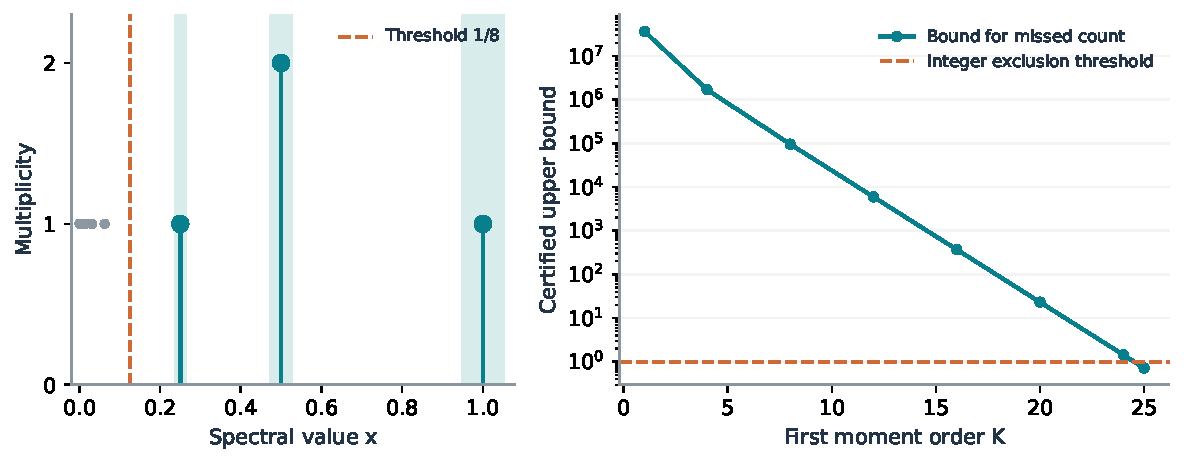
\includegraphics[width=\linewidth]{figures/certificate_example.pdf}
 \caption{Left: the exact model, with proposed intervals shaded and the
 threshold marked. Several tail points are displayed, but the calculation
 uses the whole tail. Right: the no-missing bound decreases below one at
 $K=25$. Local integer counts can already be determined at smaller $K$;
 certifying completeness is a separate requirement.}
 \label{fig:certificate}
\end{figure}

The same program verifies valid moment enclosures rounded to 36 decimal
places. It also verifies those enclosures after signed $10^{-20}$
perturbations of the candidate centers. Deliberately omitting the $1/2$
cluster fails the certificate, as do coarse moment enclosures rounded to
16 decimal places. A failed certificate is inconclusive about the
mathematical statement; it means that these particular sufficient bounds
do not prove it. In the omitted-cluster case, the proposed completeness
statement is in fact false.

The verifier accepts a JSON file containing centers, radii, a positive
integer $K$, a threshold, and a midpoint/error pair for every needed moment.
It forms the residual and count polynomials, evaluates their linear
moment functionals, and performs the interval and integer tests.
Every decision uses Python's \texttt{fractions.Fraction}. The program
rejects binary floating inputs and non-integer values of $K$.
It does not use a numerical root solver or invert a moment matrix.

\subsection{A zeta illustration, with its numerical status made explicit}

The separate program \texttt{code/zeta\_demo.py} applies the formulas to
the scaled nodes $y_n=200/(\tfrac14+\gamma_n^2)$.
It computes logarithmic Taylor coefficients of $H(200w)$ by discrete
Cauchy extraction on $|w|=1/16$, using 100-decimal-digit arithmetic and
96- and 128-point grids. Moments are obtained from the completed zeta
function, not from a truncated list of zeros. A call reporting the first
zero is used only for a diagnostic comparison.

With
\[
 K=16,\qquad a=0.99979776674462794831,\qquad
 r=0.05,\qquad \tau=0.7,
\]
the illustrative results are
\begin{center}
\begin{tabular}{@{}lr@{}}
\toprule
Quantity & Numerical value\\
\midrule
$p_{16}$ & $0.996772251654086920874827$\\
$p_{17}$ & $0.996568982997367045027571$\\
$p_{18}$ & $0.996366681112969093653953$\\
Residual $R_{16}$ & $9.25323237789\cdot10^{-7}$\\
Count estimate $S$ & $1.00003019414010$\\
Formula for count-error radius $CR_{16}$ & $0.000668452280241$\\
Formula for missed-count bound & $0.111374257031$\\
\bottomrule
\end{tabular}
\end{center}
The inverse-coordinate interval corresponds to the ordinate interval
$(13.7935812554,14.5024529500)$, and the threshold corresponds to height
$16.8956883765$. Were the input moment values accompanied by sufficiently
tight certified enclosures, these margins would certify exactly one zero
in that interval and no other positive-ordinate zero below the height.

This run is \textbf{a numerical illustration, not a certified zeta-zero
count}. The \texttt{mpmath} special-function evaluations have not been
enclosed by rigorous ball arithmetic. Agreement between grids cannot
replace such enclosures. The general theorem is proved independently of
this run; the preceding infinite-tail model is checked exactly.

For clarity, the quadrature discretization itself has a simple analytic
bound. If $M>j$ samples are used on radius $R$ and $q=p_1R<1$, then the
exact-arithmetic extracted moment obeys
\[
 |\widetilde p_j-p_j|\le p_1^j\frac{q^M}{1-q^M}.
\]
Indeed $[w^n]\log H(w)=(-1)^{n-1}p_n/n$, $p_n\le p_1^n$, and the
discrete sum aliases only indices $j+\ell M$. In this numerical run
$q\approx0.2887$ and $|H(200w)-1|\le e^q-1<1$, which justifies the
principal logarithm on the contour. The reported evaluations of the
analytic alias bound are still numerical values, not outward-rounded
certified upper endpoints.

\subsection{Exact determinant and surgery checks}

\texttt{code/determinant\_verify.py} uses exact integer determinants and gcds.
It checks Cauchy--Binet, all maximal minors, and the asserted bounds for the
four rank-two equality matrices and the rank-three complementary example.
Their Gram determinants are $24,12,8,7,24$. An optional finite enumeration
of 19,600 unit-minor normal-form triples provides an additional diagnostic;
the proof of Theorem~\ref{thm:determinant} does not rely on that enumeration.

\texttt{code/surgery\_verify.py} checks the exact rational Newton identities,
the positive disjoint root brackets, and the vanishing of the first three
coefficients of the numerator-minus-denominator polynomial in $t^2$ for
the sine-product example of Section~\ref{sec:surgery}. Thus the finite
algebra giving Taylor agreement through order five is independently
reproducible. The infinite-product statements are proved in the text.

\subsection{A practical formalization route}

No new theorem in this note is represented as already checked by Lean.
The exact programs are ordinary executable arithmetic; they are neither
kernel proofs of the analytic arguments nor a rebuild of the upstream
development. A reasonable Lean implementation would proceed in the
following order.

\begin{enumerate}
\item Formalize the four- and five-label integer Pl\"ucker lemmas. Their
proofs require elementary inequalities, finite case splits, and a modulo-three
double count. Lift them through finite incidence sums, Cauchy--Binet and
complementary minors to Theorem~\ref{thm:determinant}.
\item Prove the rational polynomial identities for $P,L_i,Q_i$ and a
finite-support version of Theorem~\ref{thm:residual}. The noise propagation
and integer-rounding corollary are algebraic and order-theoretic.
\item Prove the pointwise Taylor-remainder estimate for $h_i$ on a positive
interval, then pass from finite sums to a summable positive spectrum using
the boundedness $x_n\le p_1$.
\item Connect the completed zeta product and the symmetry quotient to the
standard Mathlib zeta function, using the upstream RH theorem only at the
zero-reality step. A rigorous numerical front end must supply certified
moment enclosures before the rational checker can certify actual zeta data.
\item Formalize the surgery construction either through the local inverse
theorem or through Newton identities and polynomial endpoint signs.
The latter has a small finite certificate interface.
\end{enumerate}

\section{What is proved, and what remains a research claim}

The results in this note have complete mathematical proofs. The spectral
certificate is unconditional for a positive summable integer spectrum;
its zeta specialization uses RH. The determinant bound and finite-factor
surgery theorem are independent of RH. Exact rational examples check the
finite arithmetic, and separate mathematical reviews checked the key
constant calculations, incidence counts, normalization, and boundary cases.
The note has not undergone external peer review.

The proposed novelty is specific: the explicit infinite-tail cluster
certificate and its error/termination theorem; the aggregate
squared-minor bound with a penalty for vanishing minors; and the particular
balanced real-zero surgery preserving an exact finite jet and the eventual
zero-counting function. The ingredients are classical. Targeted primary
literature searches identified close results and are discussed in the
relevant sections. They cannot establish that no equivalent formulation
has appeared elsewhere.

These statements do not resolve global simplicity, pair correlation,
the Lindel\"of hypothesis for unrelated $L$-function families, or a broader
version of GRH. They are concrete proved results and reusable certificates
derived from the two supplied sources, with their dependencies and
computational limits specified.

\begin{thebibliography}{99}
\small
\raggedright
\bibitem{repo}
L. Sernau and collaborators, \emph{grh-lean}, repository and readable-edition
README, inspected 26 November 2026 at commit
\nolinkurl{72fead102f663d5c7a407964a13dc0cf9d977207}.
\url{https://github.com/lsernau/grh-lean}.

\bibitem{guide}
The same repository, \emph{Reading guide}, \texttt{grh/GUIDE.md}, pinned commit above.
\href{https://github.com/lsernau/grh-lean/blob/72fead102f663d5c7a407964a13dc0cf9d977207/grh/GUIDE.md}{Permanent source link}.

\bibitem{statements}
The same repository, \texttt{grh/src/Statements.lean} and
\texttt{grh/src/Main.lean}, pinned commit above.
\href{https://github.com/lsernau/grh-lean/blob/72fead102f663d5c7a407964a13dc0cf9d977207/grh/src/Statements.lean}{Statements};
\href{https://github.com/lsernau/grh-lean/blob/72fead102f663d5c7a407964a13dc0cf9d977207/grh/src/Main.lean}{proof exports}.

\bibitem{primeerror}
The same repository, \nolinkurl{grh/src/New/Reduction/Zeros/PrimeError.lean},
especially \texttt{isPolar\_primeRemainder}.
\href{https://github.com/lsernau/grh-lean/blob/72fead102f663d5c7a407964a13dc0cf9d977207/grh/src/New/Reduction/Zeros/PrimeError.lean}{Permanent source link}.

\bibitem{mainineq}
The same repository, \nolinkurl{grh/src/New/Reduction/MainInequality.lean},
especially \texttt{star\_inequality}.
\href{https://github.com/lsernau/grh-lean/blob/72fead102f663d5c7a407964a13dc0cf9d977207/grh/src/New/Reduction/MainInequality.lean}{Permanent source link}.

\bibitem{criterion}
The same repository, \nolinkurl{grh/src/New/Reduction/Zeros/Criterion.lean},
especially \texttt{LFunction\_ne\_zero\_of\_primeRemainder\_le}.
\href{https://github.com/lsernau/grh-lean/blob/72fead102f663d5c7a407964a13dc0cf9d977207/grh/src/New/Reduction/Zeros/Criterion.lean}{Permanent source link}.

\bibitem{onesided}
The same repository, \nolinkurl{grh/src/New/Reduction/OneSidedBound.lean}.
\href{https://github.com/lsernau/grh-lean/blob/72fead102f663d5c7a407964a13dc0cf9d977207/grh/src/New/Reduction/OneSidedBound.lean}{Permanent source link}.

\bibitem{wiki}
Wikipedia contributors, \emph{Riemann hypothesis}, version accessed
26 November 2026.
\url{https://en.wikipedia.org/wiki/Riemann_hypothesis}.
Used for orientation and the status description; source-level mathematical
claims are tied to the pinned repository.

\bibitem{dlmf}
NIST Digital Library of Mathematical Functions, Section 25.4,
\emph{Reflection formulas}, especially equations 25.4.3--25.4.4.
\url{https://dlmf.nist.gov/25.4}.

\bibitem{cardon}
D. A. Cardon and S. de Gaston Roberts,
\emph{An equivalence for the Riemann Hypothesis in terms of orthogonal
polynomials}, Journal of Approximation Theory 138 (2006), no.~1, 54--64.
Author manuscript:
\url{https://mathdept.byu.edu/cardon/papers/Orthogonal_RH.pdf}.

\bibitem{decg}
Y. de Castro and F. Gamboa,
\emph{Exact reconstruction using Beurling minimal extrapolation},
Journal of Mathematical Analysis and Applications 395 (2012), 336--354.
DOI: \href{https://doi.org/10.1016/j.jmaa.2012.05.011}{10.1016/j.jmaa.2012.05.011}.
Author manuscript:
\url{https://ydecastro.github.io/research/paper4.pdf}.

\bibitem{prony}
D. Batenkov and Y. Yomdin,
\emph{On the accuracy of solving confluent Prony systems},
SIAM Journal on Applied Mathematics 73 (2013), 134--154.
\url{https://arxiv.org/abs/1106.1137}.

\bibitem{superres}
E. J. Cand\`es and C. Fernandez-Granda,
\emph{Super-resolution from noisy data},
Journal of Fourier Analysis and Applications 19 (2013), 1229--1254.
\url{https://arxiv.org/abs/1211.0290}.

\bibitem{ald}
F. Alderliefste,
\emph{A finite arithmetic test for simplicity of the Riemann zeros,
after Suzuki}, 24 November 2026, hexagon:2611.00996v1.
\url{https://hexagonmath.org/pdf/2611.00996v1}.
This is a recent research manuscript, used for comparison rather than as
an input to the proofs here.

\bibitem{generic2023}
B. Kriepke, G. M. Kyureghyan and M. Schymura,
\emph{On the size of integer programs with bounded non-vanishing
subdeterminants}, 2023.
\url{https://arxiv.org/abs/2309.03772}.

\bibitem{generic2025}
B. Kriepke and M. Schymura,
\emph{On generic $\Delta$-modular integer matrices with two rows},
version 2, 27 March 2025.
\url{https://arxiv.org/abs/2502.15394}.

\bibitem{powersums}
H. Mel\'anov\'a, B. Sturmfels and R. Winter,
\emph{Recovery from power sums}, 2021.
\url{https://arxiv.org/abs/2106.13981}.

\bibitem{eberwein}
L. Eberwein,
\emph{The truncated Weil quadratic form: inertia, visibility,
structural measurements, and no-go theorems for the Riemann Hypothesis},
October 2026 manuscript, Proposition 7.5.
\href{https://www.academia.edu/178025276/The_truncated_Weil_quadratic_form_inertia_visibility_structural_measurements_and_no_go_theorems_for_the_Riemann_Hypothesis}{Author manuscript page}.
Used only for the comparison with finite-jet nonrigidity.
\end{thebibliography}

\end{document}
